% Infografica verticale (9x16, formato storia/stato WhatsApp) per il sito
% dello Studio Medico Dottoressa Braglia. Compila con pdflatex (va benissimo
% su Overleaf); per pubblicarla su WhatsApp converti la pagina PDF in PNG/JPG
% (es. "pdftoppm -png -r 300 infografica-whatsapp.pdf pagina", o un
% convertitore online — su Overleaf basta scaricare il PDF e convertirlo).
%
% Font: Libertine (titolo, caldo, con carattere) + Lato (testo, pulito).
% Pacchetti CTAN comuni, presenti su Overleaf senza installare nulla.
\documentclass[tikz,border=0pt]{standalone}
\usepackage[T1]{fontenc}
\usepackage[utf8]{inputenc}
\usepackage{libertine}
\usepackage{lato}
\usepackage{xcolor}
\usetikzlibrary{calc}

\definecolor{studioteal}{HTML}{0D6E6E}
\definecolor{studiogrigio}{HTML}{5B6B6A}
\definecolor{studiocrema}{HTML}{FBF8F3}
\definecolor{studioscuro}{HTML}{16221F}

% Larghezza x altezza del "cartellone": 9 x 16 cm, stesso rapporto di un
% telefono (1080x1920 px). Basta cambiare questi due numeri per ridimensionare
% tutto: le coordinate sotto sono già proporzionate a queste due lunghezze.
%
% NOTA: non chiamarle \W e \H — \H è già un comando LaTeX predefinito
% (l'accento ungherese, come in "H{o}" -> ő) e ridefinirlo manda in errore
% la compilazione. Nomi per esteso, zero rischio di scontrarsi con qualcos'altro.
\newlength{\larghezza}\setlength{\larghezza}{9cm}
\newlength{\altezza}\setlength{\altezza}{16cm}

% Una croce ✚, disegnata come poligono: la usiamo sia piccola (marchio) sia
% enorme e semitrasparente (decorazione sullo sfondo).
\newcommand{\croce}[3]{
  % #1 = centro (x,y), #2 = "raggio" del braccio, #3 = colore/opacità già impostati da chi chiama
  \fill[#3] ($#1+( -0.35*#2,  1.00*#2)$) rectangle ($#1+(0.35*#2,-1.00*#2)$);
  \fill[#3] ($#1+( -1.00*#2,  0.35*#2)$) rectangle ($#1+(1.00*#2,-0.35*#2)$);
}

\begin{document}
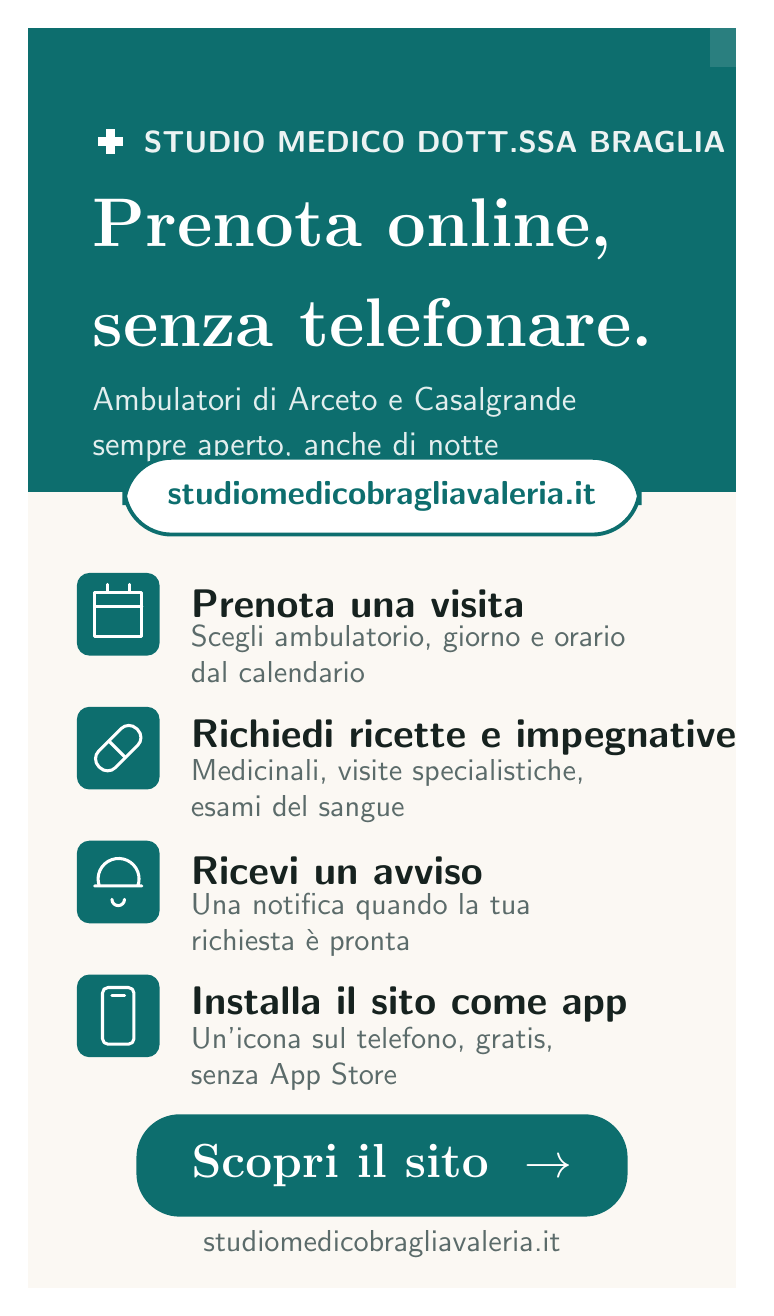
\begin{tikzpicture}[x=1cm,y=1cm]

  % ---- Sfondo (crema, caldo) --------------------------------------------
  \fill[studiocrema] (0,0) rectangle (\larghezza,\altezza);

  % ---- Fascia superiore, teal --------------------------------------------
  % Parte a 10.1cm da terra: cambia solo questo numero per allargarla o
  % stringerla (gli elementi sotto sono posizionati assumendo questo valore).
  \fill[studioteal] (0,10.1) rectangle (\larghezza,\altezza);

  % Croce grande, decorativa, appena visibile, in alto a destra
  \begin{scope}
    \clip (0,10.1) rectangle (\larghezza,\altezza);
    \croce{(9.4,17.6)}{2.1cm}{white,opacity=0.12}
  \end{scope}

  % Marchio: piccola croce + nome dello studio
  \croce{(1.05,14.55)}{0.16cm}{white}
  \node[anchor=west, text=white!92!studioteal, font=\bfseries\sffamily\fontsize{10.5}{12}\selectfont]
    at (1.35,14.55) {STUDIO MEDICO DOTT.SSA BRAGLIA};

  % Titolo, due righe — serif calda (Libertine), non il sans del resto della
  % pagina: e' l'unica riga pensata per "avere carattere" a colpo d'occhio.
  \node[anchor=north west, text=white, align=left, font=\bfseries\rmfamily\fontsize{30}{34}\selectfont]
    at (0.7,13.95) {Prenota online,\\[2pt]senza telefonare.};

  % Sottotitolo
  \node[anchor=north west, text=white!88!studioteal, align=left, font=\sffamily\fontsize{13}{16}\selectfont]
    at (0.7,11.55) {Ambulatori di Arceto e Casalgrande\\sempre aperto, anche di notte};

  % ---- Pillola con l'indirizzo del sito, a cavallo del bordo -------------
  \node[
    draw=studioteal, line width=1.4pt, fill=white, rounded corners=0.6cm,
    inner xsep=0.55cm, inner ysep=0.30cm,
    font=\bfseries\sffamily\fontsize{13}{15}\selectfont, text=studioteal
  ] at (\larghezza/2,10.05) {studiomedicobragliavaleria.it};

  % ---- Le quattro funzioni -------------------------------------------------
  \def\riga#1#2#3{%
    % #1 = coordinata y del centro dell'icona, #2 = titolo, #3 = descrizione
    \node[fill=studioteal, rounded corners=0.16cm, minimum width=1.05cm, minimum height=1.05cm]
      (icona) at (1.15,#1) {};
    \node[anchor=west, text=studioscuro, align=left, font=\bfseries\sffamily\fontsize{13.5}{16}\selectfont]
      (titolo) at (1.95,#1+0.14) {#2};
    \node[anchor=north west, text=studiogrigio, align=left, font=\sffamily\fontsize{10.5}{13}\selectfont]
      at (1.95,#1-0.02) {#3};
  }

  \riga{8.55}{Prenota una visita}{Scegli ambulatorio, giorno e orario\\dal calendario}
  \riga{6.85}{Richiedi ricette e impegnative}{Medicinali, visite specialistiche,\\esami del sangue}
  \riga{5.15}{Ricevi un avviso}{Una notifica quando la tua\\richiesta è pronta}
  \riga{3.45}{Installa il sito come app}{Un'icona sul telefono, gratis,\\senza App Store}

  % Icone (linee bianche sopra i quadratini teal disegnati da \riga)
  % Calendario
  \begin{scope}[shift={(1.15,8.55)}, white, line width=1.1pt, line cap=round, line join=round]
    \draw (-0.30,-0.28) rectangle (0.30,0.28);
    \draw (-0.30,0.10) -- (0.30,0.10);
    \draw (-0.14,0.28) -- (-0.14,0.38);
    \draw (0.14,0.28) -- (0.14,0.38);
  \end{scope}
  % Capsula (medicinale)
  \begin{scope}[shift={(1.15,6.85)}, rotate=45]
    \draw[white, line width=1.1pt, rounded corners=0.14cm] (-0.34,-0.15) rectangle (0.34,0.15);
    \draw[white, line width=1.1pt] (-0.02,-0.15) -- (-0.02,0.15);
  \end{scope}
  % Campanella (notifica)
  \begin{scope}[shift={(1.15,5.15)}, white, line width=1.1pt, line cap=round, line join=round]
    \draw (-0.24,-0.05) arc (200:-20:0.26cm) -- (0.30,-0.05) -- (-0.30,-0.05) -- cycle;
    \draw (-0.08,-0.22) arc (180:360:0.08cm);
  \end{scope}
  % Telefono (installa)
  \begin{scope}[shift={(1.15,3.45)}, white, line width=1.1pt, line cap=round, line join=round,
                rounded corners=0.07cm]
    \draw (-0.20,-0.36) rectangle (0.20,0.36);
    \draw (-0.08,0.26) -- (0.08,0.26);
  \end{scope}

  % ---- Invito finale -------------------------------------------------------
  \node[
    fill=studioteal, rounded corners=0.55cm, inner xsep=0.7cm, inner ysep=0.38cm,
    font=\bfseries\rmfamily\fontsize{16}{19}\selectfont, text=white
  ] (cta) at (\larghezza/2,1.55) {Scopri il sito \ $\rightarrow$};

  \node[anchor=north, text=studiogrigio, font=\sffamily\fontsize{10.5}{13}\selectfont]
    at (\larghezza/2,0.85) {studiomedicobragliavaleria.it};

\end{tikzpicture}
\end{document}
